\begin{figure}[h!]
    \centering
    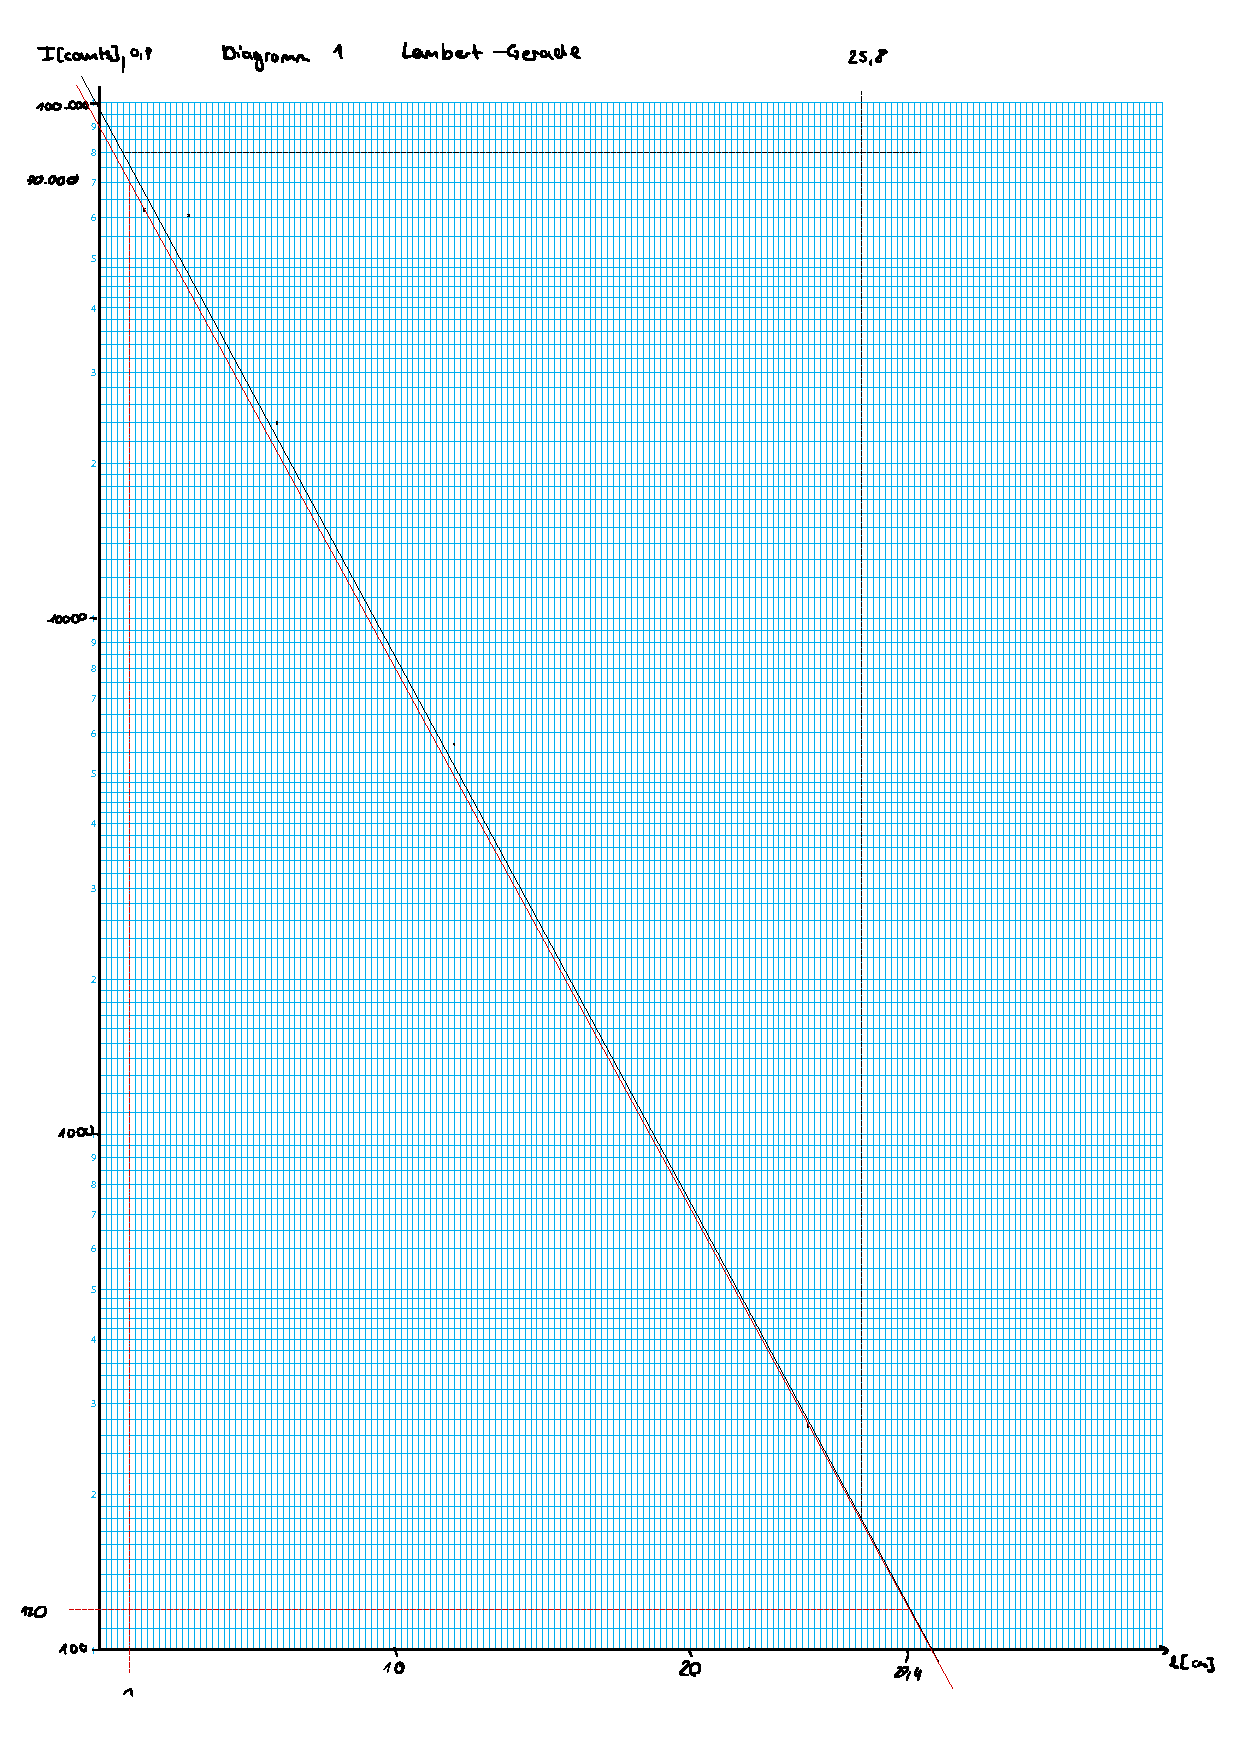
\includegraphics[page=1, width=0.95\textwidth,]{Netzpapiere_BiotechII.pdf}
    \caption{Diagramm 1}
\end{figure}
\newpage
\begin{figure}[h!]
    \centering
    \includegraphics[page=2, width=0.95\textwidth,]{Netzpapiere_BiotechII.pdf}
    \caption{Diagramm 2}
\end{figure}
\newpage
\begin{figure}[h!]
    \centering
    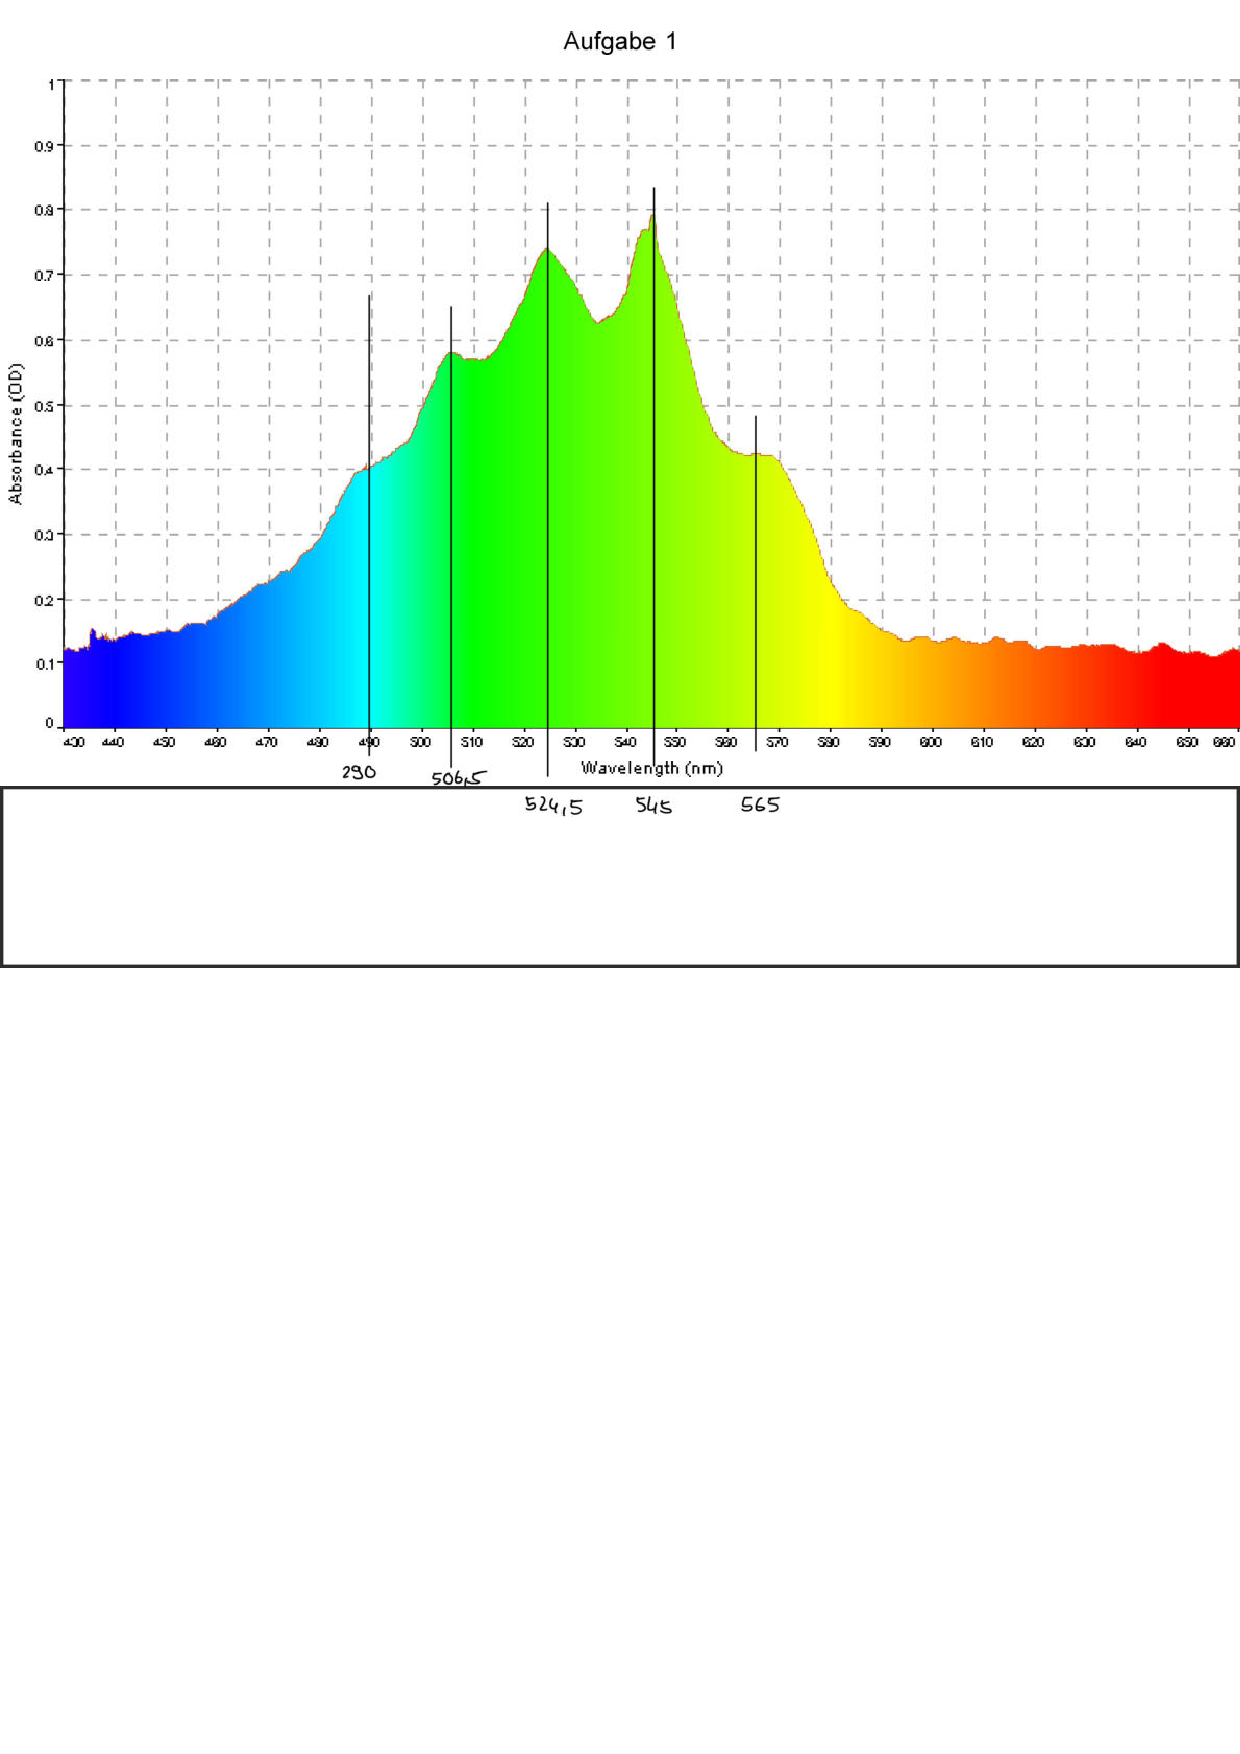
\includegraphics[page=1, width=0.95\textwidth,]{Marci Nr1.2.pdf}
    \caption{Druck Absorptionsspektrum}
\end{figure}
\newpage


\section{Vorbemerkung}
Das Gitterspektromer wiß im Verlauf der Durchführum mehrmals Fehlerhafte Messungen auf, weshalb der Intensitätswert für die 3 cm Küvette nicht verwendet wird.

\subsection{Ergänzung Messprotokoll Aufgabe 2}
\begin{table}[h!]
    \centering
    \textbf{Ergänzung Tabelle 2} \\ \smallskip
    \begin{tabular}{c c c c c}
        
        \toprule 
        Messung & Mittelwert Intensität $\overline{I}$[counts] & Abweichung $\sigma$\\
        \midrule
        1,5 cm & 63430 & 30 \\
        3 cm & 61555 & 6 \\
        6 cm & 23997 & 8 \\
        12 cm & 5703 & 13 \\
        24 cm & 321,7 & 1,7 \\
        \bottomrule
        
    \end{tabular}
    \caption{}
\end{table}

Zu berücksichtigen ist ebenfalls, dass die Küvetten einen
Fehler haben, wodurch das Licht nicht perfekt Beugungsfrei
durch diese geleitet wird. Deshalb muss diese, bei der 24cm Küvette mit berechnet werden. Dieser wird wird nach Gleichung \ref{eq:Ikorr} berechnet:

Daraus folgt für den Fehler:

\begin{equation}
    \Delta I_{korr} = \sqrt{(\frac{D_{mK}^2}{D_{oK}^2} \Delta I)^2 + (2\frac{I \cdot D_{mK}^2}{D_{oK}^3}\Delta D_{oK})^2 + (2 \frac{I \cdot D_{mK}}{D_{oK}2} \Delta D_{mK})^2}
\end{equation}

Daraus ergiebt sich für den korrigierten Intensitätswert der 24cm Küvette:

\[ I_{korr} = 276 \pm 3 \]

\subsection{Ergänzung Messprotokoll Aufgabe 3}

\begin{table}[h!]
    \centering
    \textbf{Ergänzung Aufgabe 3} \\ \smallskip
    \begin{tabular}{c c c c c}
        
        \toprule 
        Nr. & Intensität[counts] & Abweichung[counts] & Konzentration[$\tfrac{mol}{l} \cdot 10^{-6}$] & Fehler[$\tfrac{mol}{l} \cdot 10^{-6}$]\\
        \midrule
        $V_0$ & 62943 &  18 & $ 0 $ & 0 \\
        $V_1$  &  34240 &  30 & $62,5$ & $2,1 $\\
        $V_2$  & 18030 & 13 & $125$ & $2,6$\\
        $V_3$ & 5065 & 3 & $250$ & $2,4$\\
        $V_4$  & 513 & 3 & $500$ & $1,3$\\
        \bottomrule
        
    \end{tabular}
    \caption{}
\end{table}

Dabei wurde die Konzentration mit Gleichung \ref{eq:Konzentration} berechnet.
Für den Fehler ergibt sich:
\begin{equation}
    \Delta c_i = \frac{\tilde{c}}{V_{tot}^2}\left(V_0^2 \sum_ {j=1}^i\Delta V_j^2 + (V_{tot}- V_0)^2\Delta V_0^2\right)^{\tfrac{1}{2}}
\end{equation}

Wobei $V_j$ die einzel Volumina sind und $V_{tot} = \sum_{j=0}^i V_j$ also das Gesamtvolumen.

\section{Auswerung Lambert Gerade}
\subsection{Bestimmung $k'$}
Zu bestimmung des dekadischen Absoptionskoeffizienten $k'$ wird die Steigung der Trendgeraden aus Diagramm 1 betrachtet.
Da es sich hier um eine logarithmische Skala handelt wird folgende Formel verwendet:
\begin{equation}
    k' = \frac{\log(I_2)-\log(I_1)}{\Delta l}
\end{equation}

\[ \underline{\underline{k' = (0,1059 \pm 0,0011) \tfrac{1}{cm}}} \]

Dabei wurde $\Delta a$ berechnet durch:

\begin{equation}
    \Delta k' = k' - k'_{fehler}
\end{equation}

Wobei $k'_{fehler}$ für die Steigung der Fehlergeraden steht.

\subsection{Bestimmung $\epsilon$}

Da die Konzentration $c = 5 \cdot 10^{-5} \tfrac{mol}{l}$ der Küvetten bekannt ist.
Lässt sich der Extinktionskoeffizient $\epsilon$ mit Gleichung \ref{eq:dekAbsorp} berechnen. Der Fehler ist durch folgende Gleichung gegeben:
\begin{equation}
    \Delta \epsilon = \frac{\Delta k'}{c}
\end{equation}

Daraus ergibt sich für $\epsilon$:

\[ \underline{\underline{\epsilon = (2118 \pm 22) \tfrac{L}{mol \cdot \text{cm}}}}\]

oder


\[ \underline{\underline{\epsilon =( 2118 \pm 22) \cdot 10^3\tfrac{\text{cm}^2}{mol}}}\]

\section{Auswertung Beer Gerade}

Bei der Auswertung der Beer Geraden wurde mithilfe der Steigung $\frac{1}{c}$ c
bestimmt. Dabei gilt:

\begin{equation}
    \frac{1}{c} = \frac{\log(I_2)-\log(I_1)}{\Delta c}
\end{equation}

\[ \frac{1}{c} = 4360 \pm 50 \tfrac{l}{mol}\]

\begin{equation}
    \Delta(\frac{1}{c}) = \frac{1}{c} - (\frac{1}{c})_{fehler}
\end{equation}

\subsection{Berechnung $\epsilon$}

Daraus lässt sich nun mit Gelcihung \ref{eq:dekAbsorp} und $k' = \frac{1}{l}$ mit $l = 1,5 cm$
der Extinktionskoeffizient $\epsilon$ bestimmen.

\[ \underline{\underline{\epsilon = 2900 \pm 30 \tfrac{L}{mol \cdot \text{cm}}}}\]
oder:
\[ \underline{\underline{\epsilon = 2900 \pm 30 \cdot 10^3\tfrac{\text{cm}^2}{mol}}}\]

Das entspricht, verglichen mit dem Wert der Lambert-Geraden, eine Abweichung von $20 \sigma$.

